%%%%%%%%%%%%%%%%%%%%%%%%%%%%%%%%%%%%%%%%%%%%%%%%%%%%%%%%%%%%%%%%%%%%%%%%%%%%%%%%
%2345678901234567890123456789012345678901234567890123456789012345678901234567890
%        1         2         3         4         5         6         7         8

\documentclass[letterpaper, 10 pt]{IEEEconf}

\usepackage[utf8]{inputenc}
\usepackage[T1]{fontenc}

% The following packages can be found on http:\\www.ctan.org
%\usepackage{graphics} % for pdf, bitmapped graphics files
%\usepackage{epsfig} % for postscript graphics files
\usepackage{mathptmx} % assumes new font selection scheme installed
\usepackage{amsmath} % assumes amsmath package installed
\usepackage{amssymb}  % assumes amsmath package installed
\usepackage{algorithm}
\usepackage[noend]{algpseudocode}

\usepackage{tikz}
\usetikzlibrary{shapes.geometric, arrows, positioning, bending}

\usepackage{hyperref}


\usepackage{todonotes}
\def\tec{$^1$}

\title{\LARGE \bf An Overview of Reinforcement Learning}

\author{
  Emmanuel Madrigal \\
  \vspace{3pt}
  emmadrigal@estudiantec.cr
  \vspace{-18pt}
}


\begin{document}

\maketitle

%%%%%%%%%%%%%%%%%%%%%%%%%%%%%%%%%%%%%%%%%%%%%%%%%%%%%%%%%%%%%%%%%%%%%%%%%%%%%%%%
\begin{abstract}
	This document provides an overview of reinforcement learning, this
	is a machine learning technique which deals with the optimization of
	a reward function when the algorithm can only interact with an
	intermediary enviroment. Some general algorithms are shown and the
	most relevant frameworks are discussed. Its current challenges and
	some use cases are also presented.
\end{abstract}

\section{What is it?}

Reinforcement learning is learning what to do to maximize a numerical
reward signal. The learner is not told which actions to take, but must
discover which actions yield the most reward by trying them. In the
most interesting and challenging cases, actions may affect not only
the immediate reward but also the next situation and, through that,
all subsequent rewards. These two characteristics (trial-and-error
search and delayed reward) are the two most important distinguishing
features of reinforcement learning~\cite{sutton2018reinforcement}.

Reinforcement learning differs from supervised learning which
comprises learning from a training set of labeled examples provided by
a knowledgeable external supervisor. Each example is a description of
a situation together with a specification—the label—of the correct
action the system should take to that situation. The object of
supervised learning is for the system to extrapolate, or generalize,
its responses so it acts correctly in situations not present in the
training set. In interactive problems it is often impractical to get
examples of desired behavior that are both correct and representative
of all the situations in which the agent has to act. In uncharted
territory (where learning to be most beneficial), an agent must be
able to learn from its own experience~\cite{sutton2018reinforcement}.

Reinforcement learning is also different from what machine learning
researchers call unsupervised learning, which is typically about
finding structure hidden in collections of unlabeled
data. Reinforcement learning is trying to maximize a reward signal
instead of trying to find hidden structure. Uncovering structure in an
agent’s experience can be useful in reinforcement learning, but by
itself does not address the reinforcement learning problem of
maximizing a reward signal~\cite{sutton2018reinforcement}.

\section{What are its principles?} % Cuales son sus principios

\begin{figure}
	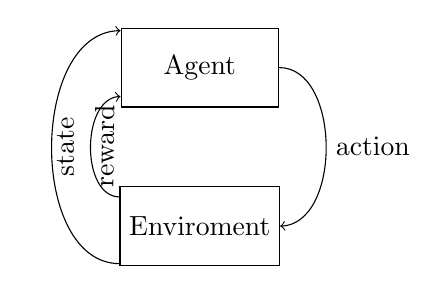
\begin{tikzpicture}[node distance=1cm]
		\node (agent) [rectangle,
			minimum width=2cm,
			minimum height=1cm,
			text centered,
			draw=black] {Agent};

		\node (env) [rectangle,
			minimum width=2cm,
			minimum height=1cm,
			text centered,
			draw=black,
			below = of agent] {Enviroment};

		\draw[bend left=90,->]  (agent.east) to node [auto] {action} (env.east);

		\draw[bend right=90,<-]  (agent.200) to node [auto, below=0.5em, sloped, anchor=center] {reward} (env.160);
		\draw[bend right=90,<-]  (agent.155) to node [auto, below=0.5em, sloped, anchor=center] {state} (env.205);
	\end{tikzpicture}
	\caption{Machine learning system}
\end{figure}

\subsection{Agent and Enviroment}

Reinforcement learning involves an interaction between an active
decision-making agent and its environment, within
which the agent seeks to achieve a goal despite uncertainty about its
environment. The agent’s actions may affect the future state of the
environment (e.g., the next chess position, the level of reservoirs of
the refinery, the robot’s next location and the future charge level of
its battery), affecting the options and opportunities available to the
agent at later times. Correct choice requires taking into account
indirect, delayed consequences of actions, and thus may require
foresight or planning. The effects of actions cannot be fully
predicted; thus the agent must monitor its environment frequently and
react appropriately. Use cases for reinforcement learning involve
explicit goals in the sense that the agent can judge progress toward
its goal based on what it can sense directly~\cite{sutton2018reinforcement}.

\subsection{Policy}

A policy defines the learning agent’s way of behaving given a
situation or state. Roughly, a policy is a mapping from perceived
states of the environment to actions to take when in those
states. Sometimes the policy may be a simple function or lookup table,
whereas in others it may involve extensive computation such as a
search process. The policy is the core of a reinforcement learning
agent in the sense that it alone suffices to determine behavior.  A
reward signal defines the goal in a reinforcement learning problem. On
each time step, the environment sends to the reinforcement learning
agent a single number called the reward. The agent’s sole aim is to
maximize the total reward it receives over the long run. The reward
signal thus defines what are the good and bad events for the
agent. They are the immediate and defining features of the problem
faced by the agent. The reward signal is the primary basis for
altering the policy; if an action selected by the policy results in a
low reward, then the policy may change to select some other action in
that situation. Reward signals may be stochastic functions of the
state of the environment and the actions taken~\cite{sutton2018reinforcement}.

\subsection{Reward and Value}

Whereas the reward signal shows what is good in an immediate sense, a
value function specifies what is good in the long run. Roughly, the
value of a state is the total amount of reward an agent can expect to
accumulate over the future, starting from that state. Whereas rewards
determine the immediate, intrinsic desirability of environmental
states, values show the long-term desirability of states after taking
into account the states that are likely to follow, and the rewards
available in those states. For example, a state might always yield a
low immediate reward but still have a high value because it is
regularly followed by other states that yield high rewards. Or the
reverse could be true.  Rewards are primary, whereas values, as
predictions of rewards, are secondary. Without rewards there could be
no values, and the only purpose of estimating values is to achieve
more reward. It is values with which we are most concerned when making
and testing decisions. Action choices are made based on value
judgments. We seek actions that bring about states of highest value,
not highest reward, because these actions result in the greatest
amount of reward for us over the long run. Unfortunately, it is much
harder to determine values than it is to determine rewards. Rewards
are given directly by the environment, but values must be estimated
and re-estimated from the sequences of observations an agent makes
over its entire lifetime. In fact, the most important component of
almost all reinforcement learning algorithms we consider is a method
for efficiently estimating values. The central role of value
estimation is arguably the most important thing we have learned about
reinforcement learning over the last few decades~\cite{sutton2018reinforcement}.

\subsection{Enviroment Model}

The fourth and final element of some reinforcement learning systems is
a model of the environment. This is something that mimics the behavior
of the environment, or that allows inferences to be made about how the
environment will behave. For example, given a state and action, the
model might predict the resultant next state and next reward. Models
are used for planning, by which we mean any way of deciding on a
course of action by considering possible future situations before they
are actually experienced. Methods for solving reinforcement learning
problems that use models and planning are called model-based methods,
as opposed to simpler model-free methods that are explicitly
trial-and-error learners—viewed as almost the opposite of planning~\cite{sutton2018reinforcement}.

\section{What algorithms exist?}

\subsection{Monte Carlo}

Recall that the value of a state is the expected return —expected cumulative future discounted reward— starting from that state. An obvious way to estimate it from experience, then, is simply to average the returns observed after visits to that state. As more returns are observed, the average should converge to the expected value. This idea underlies all Monte Carlo methods.

In particular, suppose we wish to estimate $v_\pi$(s), the value of a
states under policy $\pi$, given a set of episodes obtained by
following $\pi$ and passing through $s$. Each occurrence of states in an
episode is called a visit to $s$. Of course, $s$ may be visited multiple
times in the same episode; let us call the first time it is visited in
an episode the first visit $t$ o $s$. The first-visit MC method estimates
$v_\pi(s)$ as the average of the returns following first visits $t$ o $s$,
whereas the every-visit MC method averages the returns following all
visits $t$ o $s$.

\begin{algorithm}
	\caption{First-visit MC prediction for estimating $V \approx v_{\pi}$}
	\begin{algorithmic}[1]

		\State Initialize:
		\State $\pi \leftarrow$ policy to be evalueted
		\State $V \leftarrow$ an arbitrary state-value function
		\State $Returns \leftarrow$ an empty list, for all $s \in \mathit{S}$

		\While{True}
		\State Generate an episode using $\pi$

		\For{each state $s$ in the episode}

		\State $G \leftarrow$ the return that follows the first occurange of s
		\State Append G to $Returns(s)$
		\State $V(s) \leftarrow average(Returns(s))$
		\EndFor
		\EndWhile

	\end{algorithmic}
\end{algorithm}

As the number of visits increases, the function $V$ converges to $v_\pi(s)$;

\subsection{Q-Learning}

$$
	Q (S_t, A_t) \leftarrow Q(S_t, A_t) + \alpha \left[ R_{t+1} + \gamma \underset{a}{max} Q(S_{t+1}, a) - Q(S_t, A_t) \right]
$$

The learned action-value function $Q$ directly approximates $q_*$
which is the optimal action-value function~\cite{sutton2018reinforcement}.

\begin{algorithm}
	\caption{Q-learning for estimating $\pi \approx \pi_*$}
	\begin{algorithmic}[1]
		\State Initialize $Q(s, a)$, for all $s \in \mathit{S}$, $a \in \mathit{A}(s)$, randomly and $Q(terminal\-state, \cdot)=0$
		\If{Remaining Episodes}
		\State Initialize $S$
		\If{Remaining Steps}
		\State Choose $A$ from $S$ using policy derived from $Q$
		\State Take action $A$, observe $R, S'$
		\State $Q (S, A) \leftarrow Q(S, A) + \alpha \left[ R + \gamma \underset{a}{max} Q(S', a) - Q(S, A) \right]$
		\State $S \leftarrow S'$
		\EndIf
		\EndIf
	\end{algorithmic}
\end{algorithm}

\subsection{Deep Q-Learning~\cite{minh_dqn}}

This is an extension of Q-Learning, that combines it with artificial
neural networks. Minh et al showed in \cite{minh_dqn} how a single
reinforcement learning agent can achieve high levels of performance in
many different problems without relying on different problem-specific
feature sets.

Mnih et al.\ modified the basic Q-learning procedure in three
ways. First, they used a method called experience replay. This method
stores the agent’s experience at each timestep in a replay memory that
is accessed to perform the weight updates. After the game emulator
executed action $A_t$ in a state represented by the image stack $S_t$,
and returned reward $R_{t+1}$ and image stack $S_{t+1}$, it added the
tuple ($S_t$,$A_t$,$R_{t+1}$,$S_{t+1}$) to the replay memory. This
memory accumulated experiences over many plays of the same game. At
each time step multiple Q-learning updates—a mini-batch—were performed
based on experiences sampled uniformly at random from the replay
memory. Instead of $S_{t+1}$ becoming the new $S_t$ for the next
update as it would in the usual form of Q-learning, a new unconnected
experience was drawn from the replay memory to supply data for the
next update. Since Q-learning is an off-policy algorithm, it does not
need to be applied along connected trajectories.

Mnih et al. used a technique that brought Q-learning closer to the
simpler supervised-learning case while still allowing it to
bootstrap. Whenever a certain number, $C$, of updates had been done to
the weights $w$ of the action-value network, they inserted the
network’s current weights into another network and held these
duplicate weights fixed for the next $C$ updates of $w$. The outputs
of this duplicate network over the next $C$ updates of $w$ were used
as the Q-learning targets. Letting $\tilde{q}$ denote the output of
this duplicate network, then instead of (16.3) the update rule was:

$$
	w_{t+1}=w_t+\alpha[R_{t+1}+\gamma \underset{a}{max} \tilde{q}(S_{t+1},a,w_t)-\hat{q}(S_t,A_t,w_t)]\nabla_{w_t}\hat{q}(S_t,A_t,w_t).
$$

A final modification of standard Q-learning was also found to improve stability. They clipped the error term $R_{t+1}+\gamma \underset{a}{max} \tilde{q}\left(S_{t+1},a,w_t\right)-\hat{q}\left(S_t,A_t,w_t\right)$ so that it remained in the interval $\left[-1,1\right]$.

\subsection{Actor Critic~\cite{konda2000actor}}

The principal idea is to split the deep q-learning model in two: one
for computing an action based on a state and another one to produce
the $Q$ values of the action.

The actor takes as input the state and outputs the best action. It
essentially controls how the agent behaves by learning the optimal
policy. The critic, on the other hand, evaluates the action by
computing the value function. Those two models participate in a game
where they both get better in their own role as the time passes. The
result is that the overall architecture will learn to play to solve
the problem more efficiently than the two methods separately.

The Actor Critic has two main variants: the Asynchronous Advantage
Actor Critic (A3C) and the Advantage Actor Critic (A2C).

A3C was introduced in ~\cite{mnih2016asynchronous}. In essence, A3C
implements parallel training where multiple workers in parallel
environments independently update a global value function—hence
``asynchronous''. One key benefit of having asynchronous actors is
effective and efficient exploration of the state space.

A2C~\cite{wu_2017} is like A3C but without the asynchronous part; this
means a single-worker variant of the A3C. It was empirically found
that A2C produces comparable performance to A3C while being more
efficient.

\subsection{Double DQN~\cite{NIPS2010_3964}}

Taking the largest q value (which is noisy) as the best action to take
can lead to false positives. If non-optimal actions are regularly
given a higher Q value than the optimal best action, the learning will
be complicated.  The solution is: when we compute the Q target; we use
two networks to decouple the action choice from the target Q value
generation.

\begin{itemize}
\item Use a DQN network to select what is the best action to take for
  the next state (the action with the highest Q value).
\item Use a target network to calculate the target Q value of taking
  that action at the next state.
\end{itemize}

\subsection{Deep Deterministic Policy Gradient~\cite{lillicrap2015continuous}}

Deep Deterministic Policy Gradient (DDPG) is an algorithm which
concurrently learns a Q-function and a policy. It uses off-policy data
and the Bellman equation to learn the Q-function, and uses the
Q-function to learn the policy.

This approach is closely connected to Q-learning, and is motivated the same way: if you know the optimal action-value function $Q^*(s,a)$, then in any given state, the optimal action $a^*(s)$ can be found by solving

$$
a^*(s) = \underset{a}{arg\ max} Q^*(s,a).
$$

DDPG interleaves learning an approximator to $Q^*(s,a)$ with learning an
approximator to $a^*(s)$, and it does so in a way which is specifically
adapted for environments with continuous action spaces.

Because the action space is continuous, the function $Q^*(s,a)$ is
presumed to be differentiable with respect to the action
argument. This allows to set up an efficient, gradient-based learning
rule for a policy $\mu(s)$ which exploits that fact. Then, instead of
running an expensive optimization subroutine each time we wish to
compute $max_a Q(s,a)$, we can approximate it with $\max_a Q(s,a)
\approx Q(s,\mu(s))$.


\subsection{SARSA~\cite{rummery1994line}}

The Sarsa algorithm is an On-Policy algorithm for reinforcement learning. The
major difference between it and Q-Learning, is that the maximum reward
for the next state is not necessarily used for updating the
Q-values. Instead, a new action, and therefore reward, is selected
using the same policy that determined the original action. The name
Sarsa actually comes from the fact that the updates are done using the
quintuple $Q(s, a, r, s', a')$. Where: $s, a$ are the original state and
action, $r$ is the reward observed in the following state and $s', a'$ are
the new state-action pair.

\subsection{Other}

Other algorithms include:

\begin{itemize}
\item Proximal Policy Optimization~\cite{schulman2017proximal}.
  \item Trust-Region Policy Optimization~\cite{schulman2015trust}.
  \item Deterministic Policy Gradient~\cite{silver2014deterministic}.
  \item Generative Adversarial Imitation Learning~\cite{ho2016generative}.
  \item Hindsight Experience Relay~\cite{AndrychowiczWRS17}.
  \item Soft Actor Critic~\cite{abs-1801-01290}.
  \item Twin Delayed DDPG~\cite{dankwa2019twin}.
  \item Trust Region Policy Optimization~\cite{schulman2015trust}.
\end{itemize}


\section{Which library or frameworks are the most relevant today?}

\subsection{KerasRL}

keras-rl\cite{plappert2016kerasrl} implements some state-of-the art deep reinforcement learning
algorithms in Python and seamlessly integrates with the deep learning
library Keras.

Furthermore, keras-rl works with OpenAI Gym out of the box. This means
that evaluating and playing around with different algorithms is easy.

Implements the following algorithms:

\begin{itemize}
	\item Deep Q Learning
	\item Double DQN
	\item Deep Determenistic Policy Gradient
	\item Continous DQN
	\item Cross-Entropy Method
	\item Dueling Network DQN
	\item Deep SARSA
\end{itemize}

\subsection{Tensorforce}

Tensorforce~\cite{tensorforce} is an open-source deep reinforcement
learning framework, with an emphasis on modularized flexible library
design and straightforward usability for applications in research and
practice. Tensorforce is built on top of Google's TensorFlow framework
and requires Python 3.

\begin{itemize}
	\item Proximal Policy Optimization
	\item Trust-Region Policy Optimization
	\item Deterministic Policy Gradient
	\item Deep Q-Network
	\item Double DQN
	\item Dueling DQN
	\item Actor-Critic
	\item Advantage Actor-Critic
\end{itemize}

\subsection{Stable Baselines}

Stable Baselines~\cite{stable-baselines}, a set of implementations of
Reinforcement Learning (RL) algorithms with a common interface, based
on OpenAI Baselines. It is focused on simplicity of use and
consistency.

\begin{itemize}
	\item Advantage Actor Critic
	\item Actor Critic with Experience Replay
	\item Actor Critic using Kronecker Factored Trust Region
	\item Deep Determenistic Policy Gradient
	\item Deep Q Learning
	\item Generative Adversarial Imitation Learning
	\item Hindsight Experience Relay
	\item Proximal Policy Optimization
	\item Soft Actor Critic
	\item Twin Delayed DDPG
	\item Trust Region Policy Optimization
\end{itemize}

\subsection{TF Agents}

TF-Agents~\cite{TFAgents} is a relatively new but up-and-coming tool, again, from
Google.  TF-Agents, while newer, is typically seen as more robust and
mature. It is a framework designed for notebooks and that makes it
perfect for trying out various configurations, hyperparameters, or
environments.

\begin{itemize}
	\item Deep Q Learning
	\item Double DQN
	\item Twin Delayed DDPG
	\item REINFORCE
	\item Proximal Policy Optimization
	\item Soft Actor Critic
\end{itemize}

\section{What challenges are there?}

\subsection{Batch Off-line and Off-Policy Training}

Many systems cannot be trained on directly and need to learn from
fixed logs of the system’s behavior. Most times, we are deploying an
RL approach to replace a previous control system, and logs from that
policy are available. In future training iterations, batches of data
will be available from the most recent iteration of the control
algorithm. This setup is an off-line and off-policy training regime
where the policy needs to be trained from batches of data~\cite{deepmind2019}.

For a production system where drops in performance could be very
costly, we want to ensure that the new policy improves upon the
previous policy. Estimating the policy’s performance without running
it on the actual system is termed off-policy evaluation. Off-policy
evaluation becomes more challenging as the difference between the
policies and the resulting state distributions grows~\cite{deepmind2019}.

\subsection{Learning On the Real System from Limited Samples}

Unlike much of the research performed in deep reinforcement learning,
actual systems do not have separate training and evaluation
environments. All training data comes from the actual system, and the
agent cannot have a separate exploration policy during training as its
exploratory actions do not come for free. Instead, the agent must
perform reasonably well, and act safely throughout learning. For many
systems, this means that exploration must be limited, and the
resulting data is low-variance–very little of the state space may be
covered in the logs. In addition, since there is often only one
instance of the system approaches that instantiate hundreds or
thousands of environments to collect more data for distributed
training are usually not compatible with this setup~\cite{deepmind2019}.

Almost all of these real-world systems are slow-moving, fragile, or
expensive enough that the data they produce is costly, and policy
learning must be data-efficient. Where there are off-line logs of the
system, these might contain nowhere near the amount of data or data
coverage that current RL algorithms expect. Learning iterations on an
actual system can take a long time, as slower control frequencies
might range from 1-hour to multi-month time-steps, and reward horizons
could be on the order of months (e.g. online advertisement, drug
therapies). Even with higher-frequency control tasks, the learning
algorithm needs to learn quickly from potential mistakes without
needing to repeat them multiple times before fixing them. Thus,
learning on an actual system requires an algorithm to be both
sample-efficient and performant in its operation of the system~\cite{deepmind2019}~\cite{microsoft_research_2018}.

\subsection{Satisfying Safety Constrains}

Almost all physical systems can destroy or degrade themselves and
their environment. Considering these systems’ safety is necessary for
controlling them. Safety is important during system operation, but
also during exploratory learning phases. These could be safety
considerations either of the system itself (limiting system
temperatures, contact forces or maintaining minimum battery levels) or
of its environment (avoiding dynamic obstacles, limiting end effector
velocities). There may exist a fallback watchdog controller, which
would takeover if the learned policy violates the safety constraints,
but we consider that it should not be explicitly relied
upon~\cite{deepmind2019}.

\subsection{Partial Observability and Non-Stationarity}

Almost all real systems where we would want to deploy reinforcement
learning are partially observable. For example, on a physical system,
we likely do not have observations of the wear and tear on motors or
joints, or the amount of buildup in pipes or vents. On systems that
interact with users such as recommender systems, we have no
observations of the mental state of the users. Often, these partial
observabilities appear as non-stationarity (e.g.as a pump’s efficiency
degrades) or as stochasticity (e.g. as each robot being operated
behaves differently)~\cite{deepmind2019}.

\subsection{Unspecified and Multi-Objective Reward Functions}

Reinforcement learning frames policy learning through the lens of
optimizing a global reward function, yet most systems have
multidimensional costs to be minimized. Most times, system or product
owners do not have a clear picture of what they want to optimize. When
an agent is trained to optimize one metric, other metrics are
discovered that also need to be maintained or improved. Thus, a lot of
the work on deploying RL to real systems is in formulating the reward
function, which may be multidimensional. Because the global reward
function is generally a balance of multiple sub-goals (e.g. reducing
both time-to-target and energy use), a proper evaluation should
explicitly separate the individual components of the reward function
to better understand the policy’s tradeoffs~\cite{deepmind2019}.

\subsection{Explainability}

Another essential aspect of real systems is that they are owned and
operated by humans, who need to be reassured about the controllers’
intentions and require insights regarding failure cases. For this
reason, policy explainability is important for real-world
policies. Especially where the policy might find an alternative and
unexpected approach to controlling a system, understanding the longer
term intent of the policy is important for obtaining stakeholder
buy-in. In the event of policy errors, being able to understand the
error’s origins a posteriori is essential~\cite{deepmind2019}.

\subsection{Multi-task Learning}

To achieve general AI, an agent should be able to perform many types
of tasks, rather than specializing in just one. The core of this
challenge is scalability. It should not take 1000 times as many
samples or hours of computation time to learn 1000 different tasks
than to learn one single task. Instead, an AI agent should build up a
library of general knowledge and learn general skills that can be used
across a variety of tasks. Besides being scalable, an AI that learns
general skills can also quickly adapt to unfamiliar tasks, enabling
consistent performance in dynamic
environments~\cite{microsoft_research_2018}.

\subsection{Learning to Remember}

For many real-world tasks, an observation only captures a minor part
of the full environment state that determines the best action. In such
partially observable environments, an agent has to take into account
not just the current observation, but also past observations to
determine the best action.

For example, consider an intelligent agent in the workplace that helps
a company support team employee carrying out actions to help address a
customer issue. The human employee may ask a customer about a billing
issue. That customer might have a home phone, a mobile and an internet
account. If the human asks “What’s the outstanding balance on the
account?” the agent must remember the course of the conversation to
understand which account the human refers to.

Remembering everything in a conversation, however, makes learning a
good policy intractable. As humans speak we move from topic-to-topic,
changing the subject and looping back again. Some information is very
important whereas other information is more tangential. Hence, the
challenge is to learn a compact representation that only stores then
most salient information~\cite{microsoft_research_2018}.

\section{Use Cases}

\subsection{Resources Management in Computer Clusters}

Designing algorithms to allocate limited resources to different tasks
is challenging and requires human-generated
heuristics. In~\cite{mao2016resource} the authors showed how to use RL
to automatically learn to allocate and schedule computer resources to
waiting jobs, with the objective to minimize the average job slowdown.

They formulated the state space as the current resources allocation
and the resources profile of jobs. For action space, they used a trick
to allow the agent to choose more than one action at each time
step. Reward was the sum of $-1/duration\_of\_the\_job$ over all the
jobs in the system. Then they combined REINFORCE algorithm and
baseline value to calculate the policy gradients and find the best
policy parameters that give the probability distribution of actions to
minimize the objective. See
\href{https://github.com/hongzimao/deeprm}{this repository} for the
implentation.

\subsection{Traffic Light Control}

In~\cite{arel2010reinforcement}, researchers tried to design a traffic
light controller to solve the congestion problem. Tested only on
simulated environment though, their methods showed superior results
than traditional methods and shed a light on the potential uses of
multi-agent RL in designing traffic system.

They put five agents in the five-intersection traffic network, with an
agent at the central intersection to control traffic signaling. The
state was defined as an eight-dimensional vector with each element
representing the relative traffic flow of each lane. Eight choices
were available to the agent, each representing a phase combination,
and they defined the reward function as a reduction in the delay
compared with earlier time step. The authors used DQN to learn the Q
value of the {state, action} pairs.

\subsection{Robotics}

Robotics is an area where reinforcement learning has shown a lot of
promise. A general survey can be found
in~\cite{kober2013reinforcement}. In particular,~\cite{levine2016end}
trained a robot to learn policies to map raw videno images to the
robot’s actions. They fed the RGB images to a CNN and outputs were the
motor torques. The RL component was the guided policy search to
generate training data that came from its own state distribution.

\subsection{Personalized Recommendations}

Previous work of news recommendations faced several challenges
including the changing dynamic of news, users get bored and Click
Through Rate cannot show the retention rate of users. Guanjie et
al.~have applied RL in news recommendation system to combat the
problems in~\cite{zheng2018drn}.

They constructed four categories of
features:
\begin{itemize}
	\item User features
	\item Context features as the state features of the environment
	\item User-news features
	\item News features as the action features.
\end{itemize}

The four features were input to the Deep Q-Network (DQN) to calculate
the Q-value. The agent chose a list of news to recommend based on the
Q-value, and the user’s click on the news was a part of the reward the
RL agent received.

\subsection{Bidding and Advertising}

Researchers from Alibaba Group published~\cite{jin2018real} and
claimed that their distributed cluster-based multi-agent bidding
solution (DCMAB) has achieved promising results and thus they plan to
conduct a live test in Taobao platform.

Taobao ad platform is a place for merchants to place a bid
to display ad to the customers. This could be a multi-agent problem
because the merchants are bidding against each other and their actions
are interrelated. In the paper, merchants and customers were clustered
into different groups to reduce computational complexity. The state
space of the agents showed the cost-revenue status of the agents,
action space was the bid (continuous), and reward was the revenue
caused by the customer cluster.

\subsection{Games}

RL is so well known these days because it is the mainstream algorithm
used to solve different games and sometimes achieve superhuman
performance.

The most famous one must be AlphaGo~\cite{silver2016mastering} and
AlphaGo Zero~\cite{silver2017alphago}. AlphaGo, trained with countless
human games, already achieved superhuman performance by using value
network and Monte Carlo tree search (MCTS) in its policy network. Yet,
the researchers later on thought back and tried a purer RL approach —
train it from scratch. The researchers let the new agent, AlphaGo
Zero, played with itself and beat AlphaGo 100–0.

\subsection{Deep Learning}

More and more attempts to combine RL and other deep learning
architecture can be seen, and they showed impressive results.

One of the most influential work in RL is the pioneering work of
DeepMind to combine CNN with RL~\cite{minh_dqn}. By doing so, the
agent can “see” the environment through high-dimensional sensory and
then learn to interact with it.

RL and RNN is another combinations people used to try a novel
idea. RNN is a neural network that has “memories”. When joint with RL,
RNN gives the agents’ ability to memorize things. For
example,~\cite{hausknecht_2015} joint LSTM with RL to create Deep
Recurrent Q-Network (DRQN) to play Atari 2600
games. In~\cite{zhou2017optimizing} the authors also used RNN and RL
to solve chemical reaction optimization problem.

DeepMind showed~\cite{ganin_2018} how to use generative models and RL to generate
programs. In the model, the adversarially trained agent used the
signal as rewards to improve the actions, instead of propagating the
gradients to the input space as in the GAN training.

\addtolength{\textheight}{-9.5cm}   % This command serves to balance the column lengths
% on the last page of the document manually. It shortens
% the textheight of the last page by a suitable amount.
% This command does not take effect until the next page
% so it should come on the page before the last. Make
% sure that you do not shorten the textheight too much.

\bibliographystyle{ieeetr}
\bibliography{bibliography}

\end{document}
